% Chapter 2: Introduction
\chapter{Introduction}
\label{ch:introduction}

\section{Background}
\label{sec:background}

The internet economy has evolved dramatically over the past three decades. What began as a platform for information sharing has transformed into a complex ecosystem of APIs, web services, SaaS platforms, and increasingly, autonomous AI agents. This evolution has created new monetization challenges that traditional payment systems are ill-equipped to address.

\subsection{The Evolution of Web Monetization}

Web monetization has progressed through several distinct phases:

\begin{figure}[ht]
\centering
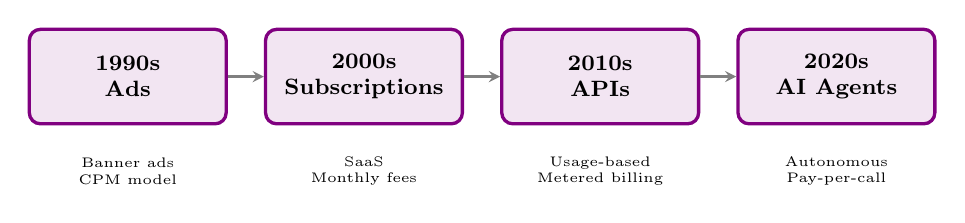
\begin{tikzpicture}[
    era/.style={
        rectangle,
        rounded corners=4pt,
        minimum width=2.5cm,
        minimum height=1.2cm,
        draw=violet,
        line width=1.2pt,
        fill=violet!10,
        font=\footnotesize\bfseries,
        align=center
    },
    desc/.style={
        rectangle,
        minimum width=2.5cm,
        font=\tiny,
        align=center
    },
    arrow/.style={->, >=stealth, thick, gray}
]

\node[era] (e1) at (0,0) {1990s\\Ads};
\node[era] (e2) at (3,0) {2000s\\Subscriptions};
\node[era] (e3) at (6,0) {2010s\\APIs};
\node[era] (e4) at (9,0) {2020s\\AI Agents};

\node[desc] at (0,-1.2) {Banner ads\\CPM model};
\node[desc] at (3,-1.2) {SaaS\\Monthly fees};
\node[desc] at (6,-1.2) {Usage-based\\Metered billing};
\node[desc] at (9,-1.2) {Autonomous\\Pay-per-call};

\draw[arrow] (e1) -- (e2);
\draw[arrow] (e2) -- (e3);
\draw[arrow] (e3) -- (e4);

\end{tikzpicture}
\caption{Evolution of web monetization models}
\label{fig:monetization-evolution}
\end{figure}

Each transition has increased the granularity and automation of payments:

\begin{enumerate}
    \item \textbf{Advertisement Era (1990s)}: Free content supported by display advertising. Payments flow from advertisers to publishers based on impressions.

    \item \textbf{Subscription Era (2000s)}: Fixed monthly fees for access to services. Simple but inflexible---users pay for unused capacity while heavy users are subsidized.

    \item \textbf{API Era (2010s)}: Usage-based pricing where customers pay for what they consume. Requires complex metering, billing cycles, and invoice processing.

    \item \textbf{AI Agent Era (2020s)}: Autonomous agents making real-time purchasing decisions. Requires instant, machine-readable payment flows with no human intervention.
\end{enumerate}

\subsection{The Problem with Traditional Payments}

Traditional payment systems were designed for human-initiated, high-value transactions. They exhibit several characteristics that make them unsuitable for the modern web:

\begin{table}[ht]
\centering
\caption{Traditional Payment System Limitations}
\label{tab:traditional-limitations}
\begin{tabular}{l l p{5cm}}
\toprule
\textbf{Characteristic} & \textbf{Traditional} & \textbf{Impact} \\
\midrule
Minimum transaction & \$0.50+ & Micropayments impossible \\
Fee structure & 2.9\% + \$0.30 & Small payments uneconomical \\
Settlement time & 1--3 days & Cash flow delays \\
Geographic limits & Regional & Global commerce barriers \\
API integration & Complex & Developer friction \\
Chargeback risk & Yes & Merchant liability \\
Machine access & Poor & AI agents cannot use \\
\bottomrule
\end{tabular}
\end{table}

\begin{infobox}[The Micropayment Problem]
For a \$0.01 API call, traditional payment processing would cost approximately \$0.30---a 3,000\% overhead. This economic reality has forced developers toward subscription models and credit systems that add complexity and friction.
\end{infobox}

\subsection{The Cryptocurrency Promise}

Cryptocurrencies theoretically solve many of these problems:

\begin{itemize}
    \item \textbf{Low Fees}: Layer 2 solutions enable sub-cent transaction costs
    \item \textbf{Instant Settlement}: Transactions confirm in seconds
    \item \textbf{Global Access}: No geographic restrictions
    \item \textbf{Programmability}: Smart contracts enable complex payment logic
    \item \textbf{No Chargebacks}: Transactions are final
\end{itemize}

However, existing cryptocurrency payment approaches have their own limitations:

\begin{table}[ht]
\centering
\caption{Cryptocurrency Payment Challenges}
\label{tab:crypto-challenges}
\begin{tabular}{l p{7cm}}
\toprule
\textbf{Challenge} & \textbf{Description} \\
\midrule
Gas Fees & Variable costs can exceed payment value \\
User Experience & Wallet connections and signing are cumbersome \\
Volatility & Price fluctuations complicate pricing \\
Fragmentation & No standard protocol for payment requests \\
Integration & Complex blockchain-specific implementations \\
\bottomrule
\end{tabular}
\end{table}

\subsection{Why Stablecoins}

\tprotocol{} focuses exclusively on stablecoin payments (primarily USDT and USDT0) for several reasons:

\begin{enumerate}
    \item \textbf{Price Stability}: 1:1 peg to USD eliminates volatility risk
    \item \textbf{Familiar Denomination}: Prices expressed in dollars are intuitive
    \item \textbf{Wide Adoption}: USDT is the most traded cryptocurrency by volume
    \item \textbf{Multi-Chain}: Available on all major blockchain networks
    \item \textbf{Regulatory Clarity}: Clearer compliance path than volatile tokens
\end{enumerate}

\begin{figure}[ht]
\centering
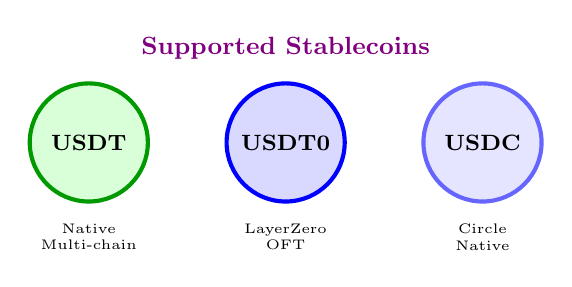
\begin{tikzpicture}[
    coin/.style={
        circle,
        minimum size=1.5cm,
        line width=1.5pt,
        font=\footnotesize\bfseries
    }
]

\node[coin, draw=green!60!black, fill=green!15] (usdt) at (0,0) {USDT};
\node[coin, draw=blue, fill=blue!15] (usdt0) at (2.5,0) {USDT0};
\node[coin, draw=blue!60, fill=blue!10] (usdc) at (5,0) {USDC};

\node[font=\tiny, align=center] at (0,-1.2) {Native\\Multi-chain};
\node[font=\tiny, align=center] at (2.5,-1.2) {LayerZero\\OFT};
\node[font=\tiny, align=center] at (5,-1.2) {Circle\\Native};

\node[font=\small\bfseries, violet] at (2.5,1.2) {Supported Stablecoins};

\end{tikzpicture}
\caption{T402 supported stablecoins}
\label{fig:stablecoins}
\end{figure}

\subsection{The Rise of AI Agents}

The emergence of AI agents capable of autonomous action introduces new requirements for payment systems. Unlike human users, AI agents:

\begin{enumerate}
    \item \textbf{Operate Programmatically}: Cannot click buttons or fill forms
    \item \textbf{Make Rapid Decisions}: May execute thousands of transactions per hour
    \item \textbf{Require Machine-Readable APIs}: Need structured data, not web pages
    \item \textbf{Have Budget Constraints}: Must evaluate costs against available funds
    \item \textbf{Need Deterministic Outcomes}: Must handle failures gracefully
\end{enumerate}

\begin{warningbox}[Agent Payment Gap]
No existing payment protocol adequately addresses the needs of autonomous AI agents. Traditional systems require human interaction; existing crypto solutions lack standardization. \tprotocol{} fills this gap.
\end{warningbox}

\section{HTTP 402: A Dormant Standard}
\label{sec:http402}

In 1997, the HTTP/1.1 specification (RFC 2068) reserved status code 402 for ``Payment Required.'' The specification noted it was ``reserved for future use,'' anticipating the eventual need for native web payments.

\begin{quote}
\textit{``This code is reserved for future use. The initial motivation for this status code is that it might be useful for digital cash or micropayment schemes.''} --- RFC 7231 \cite{rfc7231}
\end{quote}

For over 25 years, this status code remained largely unused. The technical infrastructure for secure, programmable payments simply did not exist:

\begin{itemize}
    \item No widely adopted digital currency
    \item No standardized signing schemes
    \item No programmable settlement layer
    \item No machine-readable payment protocols
\end{itemize}

The advent of blockchain technology, stablecoins, and standardized signing schemes (EIP-712, EIP-3009) has finally made the vision practical.

\subsection{Why HTTP 402}

Using HTTP 402 provides several advantages:

\begin{table}[ht]
\centering
\caption{Benefits of HTTP 402}
\label{tab:http402-benefits}
\begin{tabular}{l p{7cm}}
\toprule
\textbf{Benefit} & \textbf{Description} \\
\midrule
Standardization & Part of HTTP specification since 1997 \\
Semantic Clarity & Unambiguous meaning: payment required \\
Infrastructure & Works with existing proxies, CDNs, load balancers \\
Discoverability & Clients can detect paid resources automatically \\
Fallback & Graceful degradation for non-supporting clients \\
\bottomrule
\end{tabular}
\end{table}

\tprotocol{} activates HTTP 402 as the signaling mechanism for payment requirements, creating a standardized flow that works with existing HTTP infrastructure.

\section{Design Goals}
\label{sec:design-goals}

\tprotocol{} was designed with the following core principles:

\subsection{Minimize Trust}

The protocol minimizes trust requirements between parties:

\begin{figure}[ht]
\centering
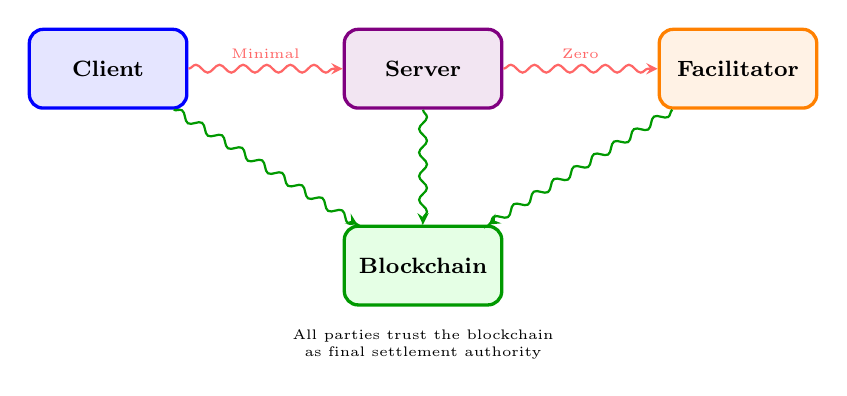
\begin{tikzpicture}[
    party/.style={
        rectangle,
        rounded corners=5pt,
        minimum width=2cm,
        minimum height=1cm,
        line width=1.2pt,
        font=\footnotesize\bfseries
    },
    trust/.style={
        ->,
        >=stealth,
        thick,
        decorate,
        decoration={snake, amplitude=0.5mm, segment length=3mm}
    }
]

\node[party, draw=blue, fill=blue!10] (client) at (0,0) {Client};
\node[party, draw=violet, fill=violet!10] (server) at (4,0) {Server};
\node[party, draw=orange, fill=orange!10] (facilitator) at (8,0) {Facilitator};
\node[party, draw=green!60!black, fill=green!10] (blockchain) at (4,-2.5) {Blockchain};

% Trust relationships
\draw[trust, red!60] (client) -- node[above, font=\tiny] {Minimal} (server);
\draw[trust, red!60] (server) -- node[above, font=\tiny] {Zero} (facilitator);
\draw[trust, green!60!black, ->] (client) -- (blockchain);
\draw[trust, green!60!black, ->] (server) -- (blockchain);
\draw[trust, green!60!black, ->] (facilitator) -- (blockchain);

\node[font=\tiny, align=center] at (4,-3.5) {All parties trust the blockchain\\as final settlement authority};

\end{tikzpicture}
\caption{Trust relationships in T402}
\label{fig:trust-model}
\end{figure}

\begin{itemize}
    \item \textbf{Client to Server}: Payment verified before resource delivery
    \item \textbf{Server to Facilitator}: Facilitator cannot redirect funds (cryptographically enforced)
    \item \textbf{All Parties}: Blockchain provides final settlement authority
\end{itemize}

\subsection{Transport Agnosticism}

Payment logic is separated from transport concerns, enabling the same payment flow across different communication protocols:

\begin{table}[ht]
\centering
\caption{Supported Transport Layers}
\label{tab:transports}
\begin{tabular}{l l p{5cm}}
\toprule
\textbf{Transport} & \textbf{Use Case} & \textbf{Description} \\
\midrule
HTTP & Web APIs & Traditional REST/GraphQL services \\
MCP & AI Tools & Model Context Protocol for LLMs \\
A2A & Agent Mesh & Agent-to-Agent communication \\
\bottomrule
\end{tabular}
\end{table}

\subsection{Chain Agnosticism}

The protocol abstracts blockchain-specific details behind a unified interface:

\begin{table}[ht]
\centering
\caption{Supported Blockchain Networks}
\label{tab:chains-intro}
\begin{tabular}{l l l}
\toprule
\textbf{Network} & \textbf{Mechanism} & \textbf{Signature} \\
\midrule
EVM Chains & EIP-3009 & ECDSA secp256k1 \\
Solana & SPL Token & Ed25519 \\
TON & Jetton & Ed25519 \\
TRON & TRC-20 & ECDSA secp256k1 \\
\bottomrule
\end{tabular}
\end{table}

\subsection{Gasless Experience}

Users pay only for the service---not for blockchain transaction fees:

\begin{infobox}[Gasless Payments]
The Facilitator sponsors all gas fees. Users sign authorizations off-chain (zero gas), and the Facilitator executes on-chain settlement. This provides a Web2-like experience while maintaining blockchain security.
\end{infobox}

\subsection{Developer Experience}

Integration should be simple. A complete server-side implementation requires minimal code:

\begin{lstlisting}[language=typescript,caption={Express.js integration example}]
import { paymentMiddleware } from "@t402/express";

app.use(paymentMiddleware({
  "GET /api/premium": {
    price: "$0.01",
    payTo: "0x..."
  }
}));
\end{lstlisting}

Client-side integration is equally straightforward:

\begin{lstlisting}[language=typescript,caption={Client-side integration example}]
import { T402Client } from "@t402/client";

const client = new T402Client({ signer });
const response = await client.fetch(
  "https://api.example.com/premium"
);
\end{lstlisting}

\section{Comparison with Alternatives}
\label{sec:comparison}

\begin{table}[ht]
\centering
\caption{Protocol Comparison}
\label{tab:protocol-comparison}
\footnotesize
\begin{tabular}{l c c c c}
\toprule
\textbf{Feature} & \textbf{T402} & \textbf{Stripe} & \textbf{Lightning} & \textbf{Request} \\
\midrule
Micropayments & \checkmark & -- & \checkmark & -- \\
No KYC & \checkmark & -- & \checkmark & \checkmark \\
Instant Settlement & \checkmark & -- & \checkmark & \checkmark \\
Stablecoin & \checkmark & -- & -- & \checkmark \\
Gasless & \checkmark & N/A & \checkmark & -- \\
AI Agent Ready & \checkmark & -- & -- & -- \\
Multi-chain & \checkmark & N/A & -- & \checkmark \\
\bottomrule
\end{tabular}
\end{table}

\section{Document Structure}
\label{sec:structure}

This whitepaper is organized as follows:

\begin{description}
    \item[Chapter 3: Architecture] presents the protocol architecture, including system components, payment flows, and trust model.

    \item[Chapter 4: Core Specifications] details data schemas, network identifiers, error codes, and protocol extensions.

    \item[Chapter 5: Payment Schemes] describes payment schemes, focusing on the ``exact'' scheme across EVM, Solana, TON, and TRON.

    \item[Chapter 6: Transport Layers] covers transport implementations for HTTP, MCP, and A2A protocols.

    \item[Chapter 7: Facilitator Service] documents the Facilitator API, self-hosting options, and operational considerations.

    \item[Chapter 8: Security Analysis] provides threat modeling, cryptographic analysis, and security recommendations.

    \item[Chapter 9: Implementation Guide] offers practical guidance with SDK examples across TypeScript, Python, Go, and Java.

    \item[Chapter 10: Use Cases] explores applications from API monetization to AI agent payments.

    \item[Chapter 11: Economics] analyzes the cost model, fee structures, and economic comparisons.

    \item[Chapter 12: Future Work] outlines planned extensions including Permit2, up-to scheme, and subscriptions.

    \item[Chapter 13: Conclusion] summarizes the protocol and provides a call to action.
\end{description}
